\documentclass[a4paper]{article}
\usepackage{cmap}
\usepackage[utf8]{inputenc}
\usepackage[T2A]{fontenc}
\usepackage[english,russian]{babel} 
\usepackage[left=15mm, top=15mm, right=15mm, bottom=42mm, nohead, nofoot]{geometry}
\usepackage{blindtext}  % рыба-текст
\usepackage{graphicx}  % изобржаения
\usepackage{float} % плавающие объекты
\usepackage{wrapfig}  % изобржаения
\usepackage{tikz} % графика
\usepackage{xcolor} % определение цветов
\usepackage{nicefrac} % красивые дроби
\usepackage{cancel} % сокращение
\usepackage{amsmath,amsfonts,amssymb} % математический пакет
\usepackage{hyperref}  % гиперссылки
\usepackage{fancybox,fancyhdr} % хедер и футер
\usepackage{listings} % код
\usepackage{accsupp}
\usepackage{caption}
\usepackage{enumitem}
\captionsetup[figure]{name=Рисунок}
\pagestyle{fancy}
\fancyhf{}
\fancyhead[L]{Лабораторная работа №3}
\fancyhead[R]{\textit{Вынужденное движение и показатели качества}}
\fancyfoot[C]{\thepage}
\headsep=8mm
\footskip=20mm

\setlist{leftmargin=1.3cm}

\definecolor{urlcolor}{HTML}{3454D1}
\definecolor{linkcolor}{HTML}{3454D1}
\hypersetup{pdfstartview=FitH, linkcolor=linkcolor, urlcolor=urlcolor, colorlinks=true}

\definecolor{strings}{rgb}{0,0.6,0}
\definecolor{comments}{rgb}{0,0.3,0}
\definecolor{numbers}{rgb}{0.5,0.5,0.5}
\definecolor{keywords}{rgb}{0.09,0.61,0.95}
\definecolor{background}{rgb}{0.97,0.97,0.97}
\newcommand{\noncopynumber}[1]{%
    \BeginAccSupp{method=escape,ActualText={}}%
    #1%
    \EndAccSupp{}%
}
\lstdefinestyle{codestyle}{
    backgroundcolor=\color{background},
    commentstyle=\color{comments},
    keywordstyle=\color{keywords},
    stringstyle=\color{strings},
    numberstyle=\tiny\color{numbers}\noncopynumber,
    basicstyle=\ttfamily\footnotesize,
    breakatwhitespace=false,
    breaklines=true,
    captionpos=b,
    inputencoding=utf8,
    keepspaces=true,
    numbers=left,
    numbersep=5pt,
    showspaces=false,
    showstringspaces=false,
    showtabs=false,
    tabsize=2,
    extendedchars=true,
    literate=
    {а}{{\cyra}}1
    {б}{{\cyrb}}1
    {в}{{\cyrv}}1
    {г}{{\cyrg}}1
    {д}{{\cyrd}}1
    {е}{{\cyre}}1
    {ж}{{\cyrzh}}1
    {з}{{\cyrz}}1
    {и}{{\cyri}}1
    {й}{{\cyrishrt}}1
    {к}{{\cyrk}}1
    {л}{{\cyrl}}1
    {м}{{\cyrm}}1
    {н}{{\cyrn}}1
    {о}{{\cyro}}1
    {п}{{\cyrp}}1
    {р}{{\cyrr}}1
    {с}{{\cyrs}}1
    {т}{{\cyrt}}1
    {у}{{\cyru}}1
    {ф}{{\cyrf}}1
    {х}{{\cyrh}}1
    {ц}{{\cyrc}}1
    {ч}{{\cyrch}}1
    {ш}{{\cyrsh}}1
    {щ}{{\cyrshch}}1
    {ъ}{{\cyrhrdsn}}1
    {ы}{{\cyrery}}1
    {ь}{{\cyrsftsn}}1
    {э}{{\cyrerev}}1
    {ю}{{\cyryu}}1
    {я}{{\cyrya}}1
    {А}{{\CYRA}}1
    {Б}{{\CYRB}}1
    {В}{{\CYRV}}1
    {Г}{{\CYRG}}1
    {Д}{{\CYR96}}1
    {Е}{{\CYRE}}1
    {Ж}{{\CYRZH}}1
    {З}{{\CYRZ}}1
    {И}{{\CYRI}}1
    {Й}{{\CYRISHRT}}1
    {К}{{\CYRK}}1
    {Л}{{\CYRL}}1
    {М}{{\CYRM}}1
    {Н}{{\CYRN}}1
    {О}{{\CYRO}}1
    {П}{{\CYRP}}1
    {Р}{{\CYRR}}1
    {С}{{\CYRS}}1
    {Т}{{\CYRT}}1
    {У}{{\CYRU}}1
    {Ф}{{\CYRF}}1
    {Х}{{\CYRH}}1
    {Ц}{{\CYRC}}1
    {Ч}{{\CYRCH}}1
    {Ш}{{\CYRSH}}1
    {Щ}{{\CYRSHCH}}1
    {Ъ}{{\CYRHRDSN}}1
    {Ы}{{\CYRERY}}1
    {Ь}{{\CYRSFTSN}}1
    {Э}{{\CYREREV}}1
    {Ю}{{\CYRYU}}1
    {Я}{{\CYRYA}}1
}

\lstset{style=codestyle}

\addto\captionsrussian{
  \renewcommand{\contentsname}
    {\centering Содержание}
}


\newlength{\tempheight}
\newcommand{\Let}{
\mathbin{\text{\settoheight{\tempheight}{\mathstrut}\raisebox{0.4\pgflinewidth}{
\tikz[baseline=0.5ex,line cap=round,line join=round] \draw (0,0) --++ (0.3em,0) --++ (0,2.3ex) --++ (-0.3em,0);
}}}}
\newcommand*\squared[1]{\tikz[baseline=(char.base)]{
            \node[shape=rectangle,draw,inner sep=4pt] (char) {#1};}}
\newcommand*\msquared[1]{\tikz[baseline=(char.base)]{
            \node[shape=rectangle,draw,inner sep=4pt] (char) {$\displaystyle #1$};}}
\newcommand{\at}{\biggr\rvert}
\newcommand{\shiftright}[3]{\makebox[#2][r]{\makebox[#1][l]{#3}}}
\newcommand{\e}{\;\text{e}}
\let\oldint\int
\def\int{\oldint\limits}
\DeclareRobustCommand{\divby}{%
  \mathrel{\vbox{\baselineskip.65ex\lineskiplimit0pt\hbox{.}\hbox{.}\hbox{.}}}%
}

\newcommand\NB{\textbf{N\kern-0.32em\textcolor{red}{B}}}

\begin{document}

\begin{titlepage}
    \begin{center}
        Федеральное государственное автономное образовательное \\ учреждение высшего образования \\[6pt]
        САНКТ-ПЕТЕРБУРГСКИЙ НАЦИОНАЛЬНЫЙ \\ ИССЛЕДОВАТЕЛЬСКИЙ УНИВЕРСИТЕТ ИТМО \\[16pt]
        Факультет систем управления и робототехники \\[26em]
        Лабораторная работа №3\\[0.5em]
        \textbf{ВЫНУЖДЕННОЕ ДВИЖЕНИЕ И ПОКАЗАТЕЛИ КАЧЕСТВА}
    \end{center}\,\\[10em]
    \begin{flushright}
        Студент: Заводин Е.Ю.\\
        Лин САУ R23 бак 1.1.1 \\[0.5em]
        Преподаватели: Перегудин А.А.\\
        Пашенко А.В.
    \end{flushright}\,\\[6em]
    \begin{center}
        {\small Санкт-Петербург \\ 2025}
    \end{center}
\end{titlepage}
\setcounter{page}{2}
\tableofcontents\newpage

\section{Вынужденное движение}\

В задании рассматриваю систему 2-го порядка, заданную уравнением 

$$
\ddot{y}+a_1\dot{y} + a_0y=a_0 u
$$\

Для этой системы составил структурную схему:

\begin{figure}[H]
    \centering
    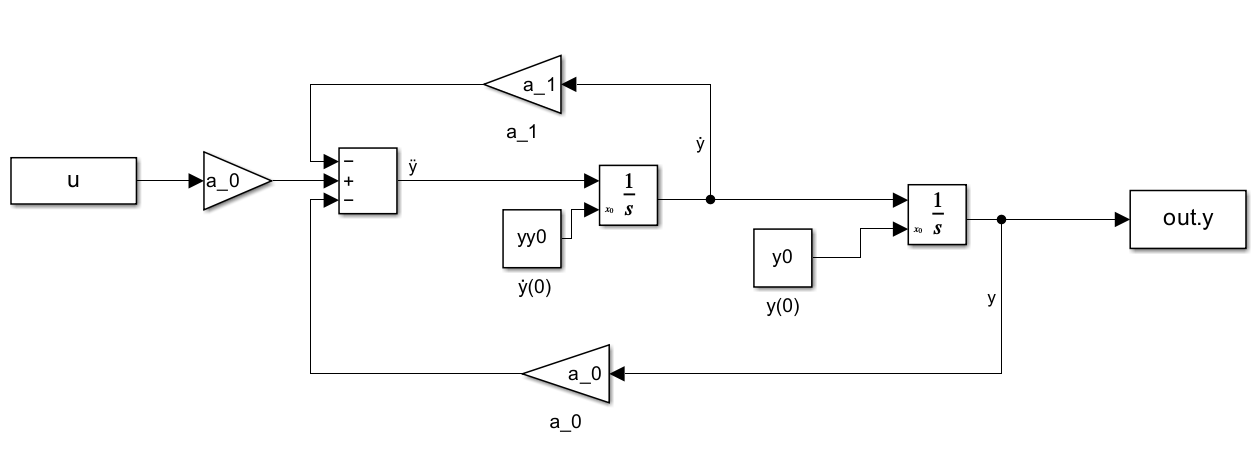
\includegraphics[width=0.75\linewidth]{ex1/scheme.png}
    \caption{Структурная схема системы первого задания}
\end{figure}\

Поочерёдно возьмём варианты входного сигнала из следующего набора параметров: $\{1.5, 0.6t, \sin{6t}\}$, а также наборы параметров $a_1, a_0$, взятые из предыдущей лабораторной работы: $\{[2, 65], [0, 64], [-2, 65]\}$. Для каждого значения из каждого набора параметров построим систему, и промоделируем её при трёх различных случаях начальных условий\

\begin{itemize}
    \item $y(0) = -1, \dot{y}(0) = 0;$
    \item $y(0) = 0, \dot{y}(0) = 0;$
    \item $y(0) = 1, \dot{y}(0) = 0.$
\end{itemize}\ 

\begin{figure}[H]
    \begin{minipage}{0.5\textwidth}
        \centering 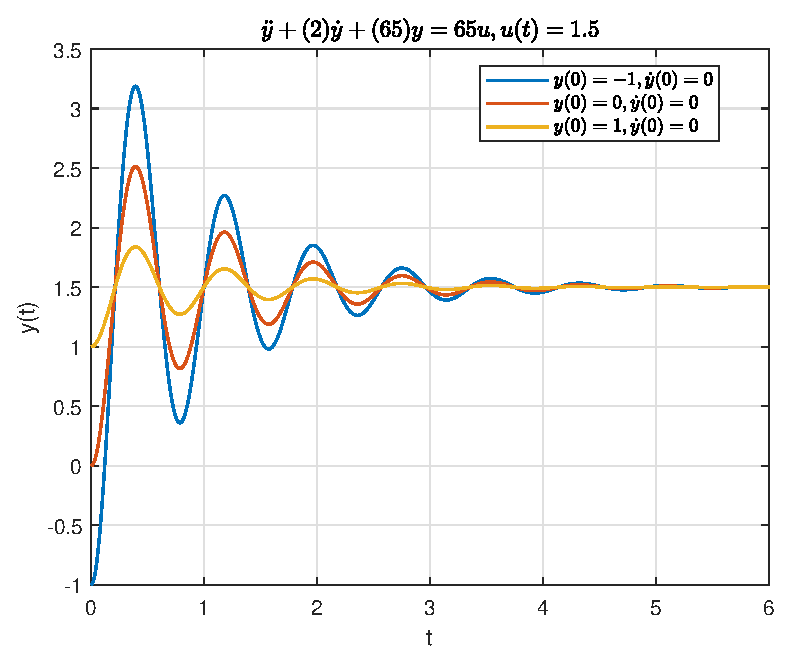
\includegraphics[width=\textwidth]{ex1/1.5_2_65}
        \caption{$a_1 = 2, a_0 = 65, u(t) = 1.5$}
    \end{minipage}\hfill
    \begin{minipage}{0.5\textwidth}
        \centering 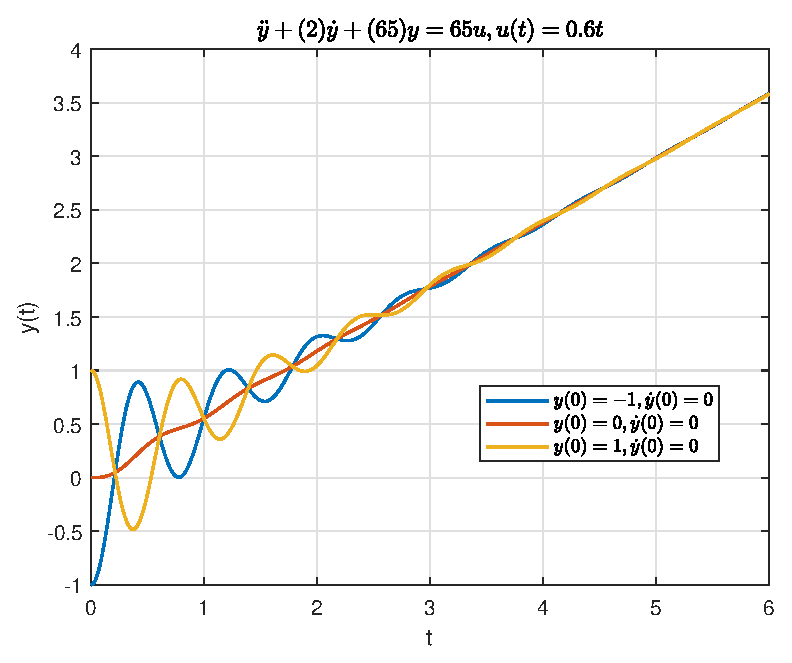
\includegraphics[width=\textwidth]{ex1/0.6t_2_65}
        \caption{$a_1 = 2, a_0 = 65, u(t) = 0.6t$}
    \end{minipage}\\[1em]
\end{figure}\noindent\

\begin{figure}[H]
    \centering
    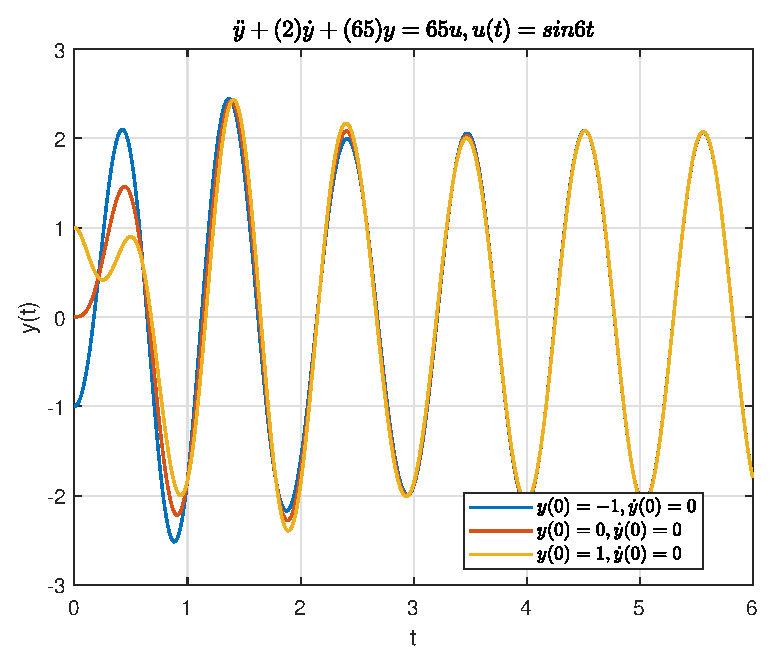
\includegraphics[width=0.6\linewidth]{ex1/sin6t_2_65.eps}
    \caption{$a_1 = 2, a_0 = 65, u(t) = \sin{6t}$}
\end{figure}\

Для первого набора параметров система асимптотически устойчива. При всех рассмотренных начальных условиях система демонстрирует схожее поведение. Видно воздействие входного сигнала -- $u(t)$ как бы накладывается на график решения системы, смещая её по оси ординат на константную величину входного сигнала (1.5) в случае $u(t) = 1.5$. В случае с $u(t) = 0.6t$ график выхода $y(t)$ начинает стремиться к наклонной прямой, которой и является график $u(t)$. При $u(t) = \sin{(6t)}$ система теряет свою асимптотическую устойчивость, становится устойчивой по Ляпунову, и сходится уже к некой гармонике.

\begin{figure}[H]
    \begin{minipage}{0.5\textwidth}
        \centering 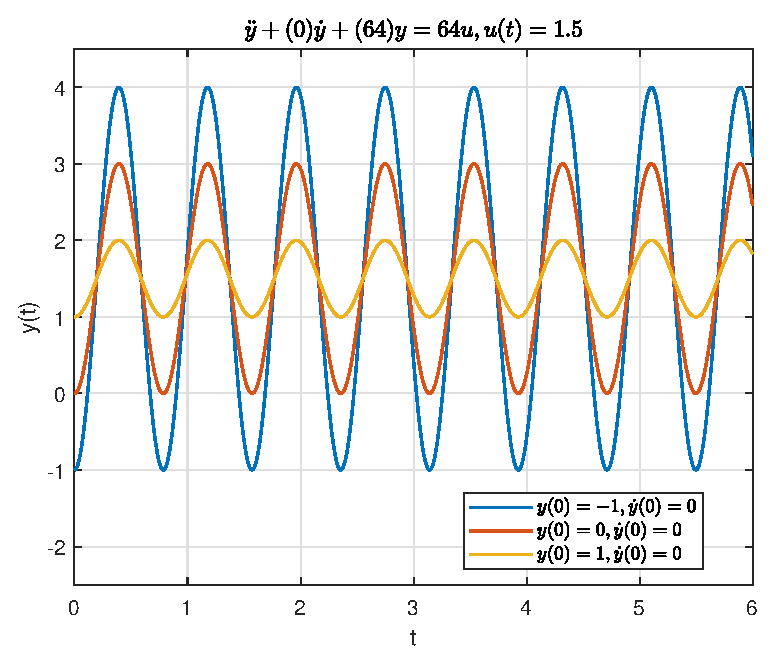
\includegraphics[width=\textwidth]{ex1/1.5_0_64.eps}
        \caption{$a_1 = 0, a_0 = 64, u(t) = 1.5$}
    \end{minipage}\hfill
    \begin{minipage}{0.5\textwidth}
        \centering 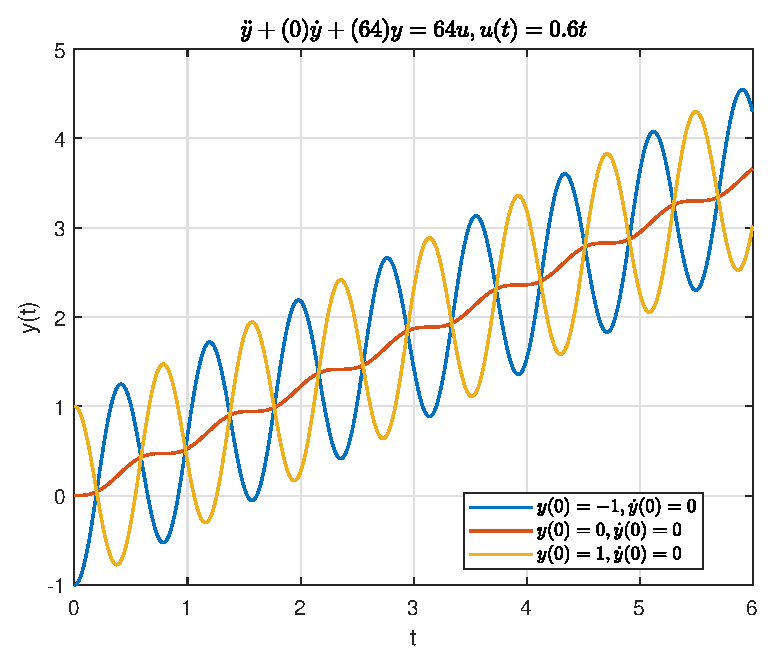
\includegraphics[width=\textwidth]{ex1/0.6t_0_64.eps}
        \caption{$a_1 = 0, a_0 = 64, u(t) = 0.6t$}
    \end{minipage}\\[1em]
\end{figure}\noindent\

\begin{figure}[H]
    \centering
    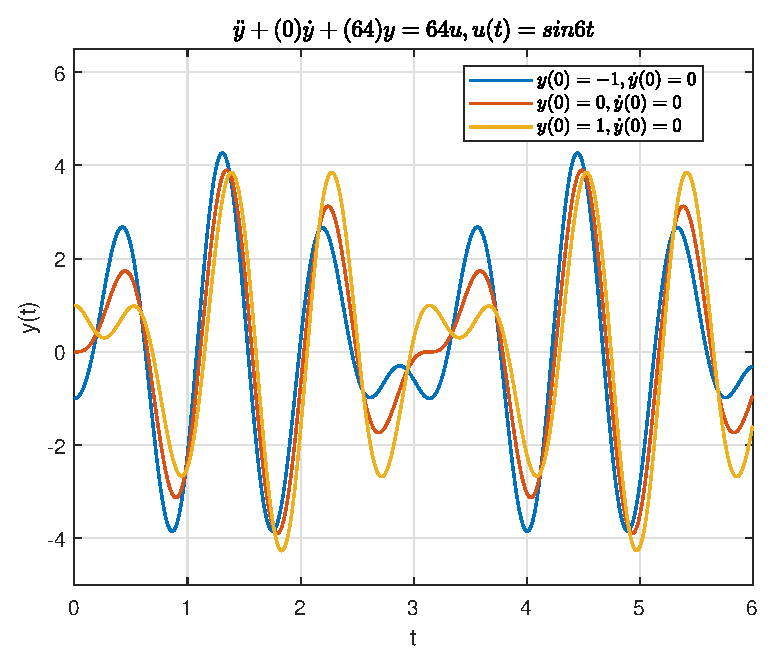
\includegraphics[width=0.6\linewidth]{ex1/sin6t_0_64.eps}
    \caption{$a_1 = 0, a_0 = 64, u(t) = \sin{6t}$}
\end{figure}\

В этом случае система в отсутствие начального воздействия является устойчивой по Ляпунову, не имеет асимптотической устойчивости. Входное воздействие вида константной функции, как и в случае с предыдущим набором параметров, смещает график выходного сигнала по оси ординат, воздействие на систему вида наклонной прямой сказывается схожим образом, однако колебания при различных начальных условиях имеют разную амплитуду, в отличие от других видов рассмотренных воздействий. В случае с гармоническим сигналом в виде входного воздействия картина чуть более интересная -- гармоники свободной и вынужденной составляющих движения накладываются друг на друга, появляется новая устойчивая гармоника с частотой 6, и период периодической функции выхода меняется.

\begin{figure}[H]
    \begin{minipage}{0.5\textwidth}
        \centering 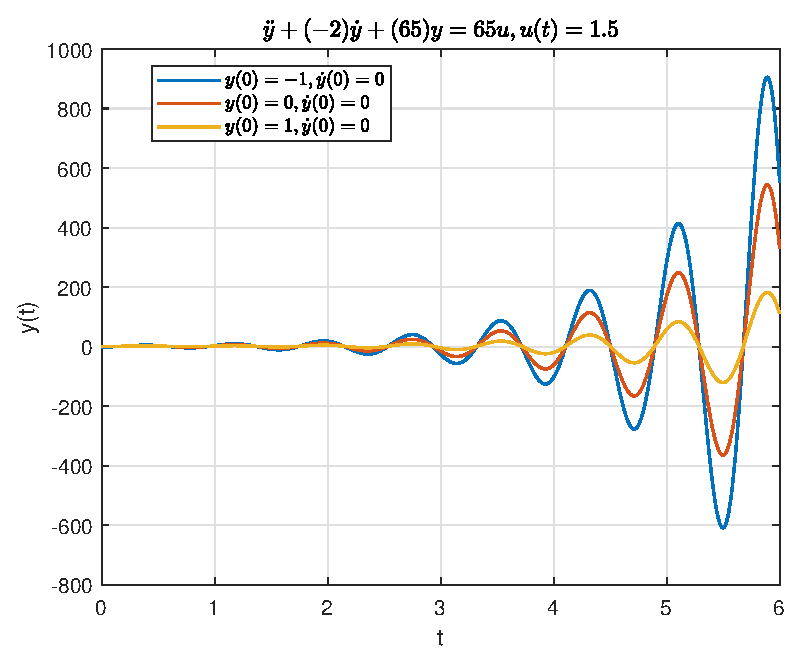
\includegraphics[width=\textwidth]{ex1/1.5_-2_65.eps}
        \caption{$a_1 = -2, a_0 = 65, u(t) = 1.5$}
    \end{minipage}\hfill
    \begin{minipage}{0.5\textwidth}
        \centering 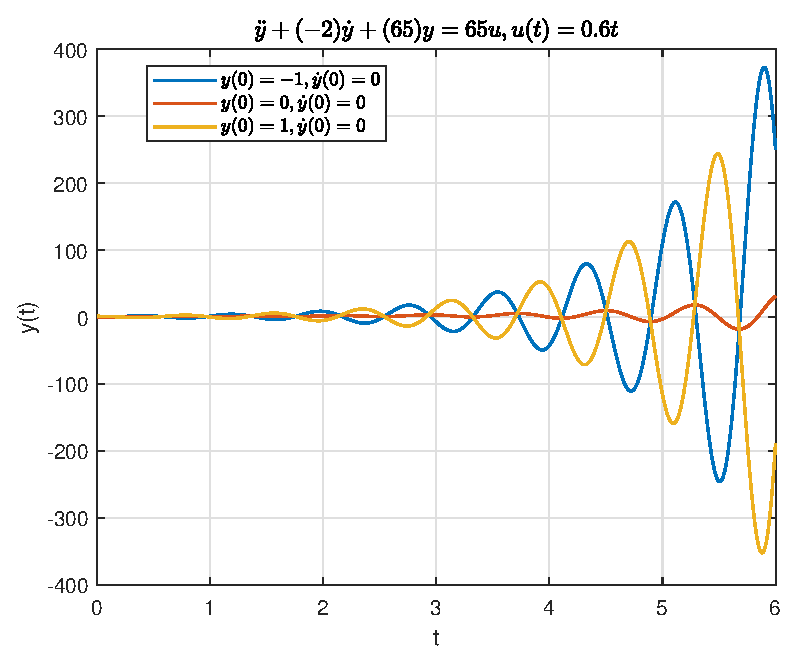
\includegraphics[width=\textwidth]{ex1/0.6t_-2_65.eps}
        \caption{$a_1 = -2, a_0 = 65, u(t) = 0.6t$}
    \end{minipage}\\[1em]
\end{figure}\noindent\

\begin{figure}[H]
    \centering
    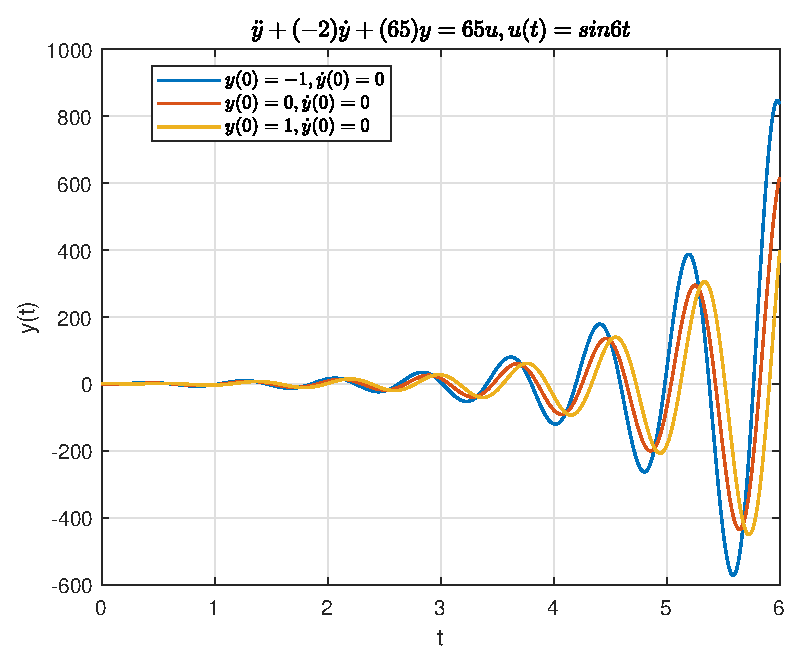
\includegraphics[width=0.6\linewidth]{ex1/sin6t_-2_65.eps}
    \caption{$a_1 = -2, a_0 = 65, u(t) = \sin{6t}$}
\end{figure}\

При третьем наборе параметров система в отсутствие входного воздействия расходится с течением времени, и воздействие вида $u(t) = 0.6t$ приводит к рассогласованию выходов системы при различных начальных условиях, а также замедляет скорость расхождения системы при нулевых начальных условиях, но в конечном счёте график всё равно уйдёт в бесконечность.

\subsection{Выводы}\

Входное воздействие влияет на выход системы, и разные входные воздействия влияют по-разному, при этом не меняя тип устойчивости системы в сравнении с соответствующими им свободными системами (с нулевым начальным воздействием)

\section{Качество переходных процессов}\

В задании рассматривается передаточная функция следующего вида:

$$
W(s) = \frac{|\lambda_1\lambda_2\lambda_3|}{(s-\lambda_1)(s-\lambda_2)(s-\lambda_3)}
$$\

В качестве исследуемых наборов полюсов $\lambda_1, \lambda_2, \lambda_3$ взяты следующие:

\begin{enumerate}
\item{$\lambda_1=-1, \lambda_2=-1, \lambda_3=-1$}
\item{$\lambda_1=-1, \lambda_2=-1, \lambda_3=-10$}
\item{$\lambda_1=-1, \lambda_2=-20, \lambda_3=-10$}
\item{$\lambda_1=-1+i, \lambda_2=-1-i, \lambda_3=-1$}
\item{$\lambda_1=-1+i, \lambda_2=-1-i, \lambda_3=-5$}
\item{$\lambda_1=-1+3i, \lambda_2=-1-3i, \lambda_3=-5$}
\item{$\lambda_1=-3+3i, \lambda_2=-3-3i, \lambda_3=-5$}
\item{$\lambda_1=-3+100i, \lambda_2=-3-100i, \lambda_3=-5$}
\end{enumerate}\

Для определения времени переходного процесса принял для всех наборов окрестность установившегося значения $\Delta_\text{П} = 0.02 \,\, (0.02\%)$, промоделировал получившиеся системы без начальных условий для каждого из наборов полюсов, в качестве входного воздействия применяя функцию Хевисайда:

\begin{figure}[H]
    \begin{minipage}{0.5\textwidth}
        \centering 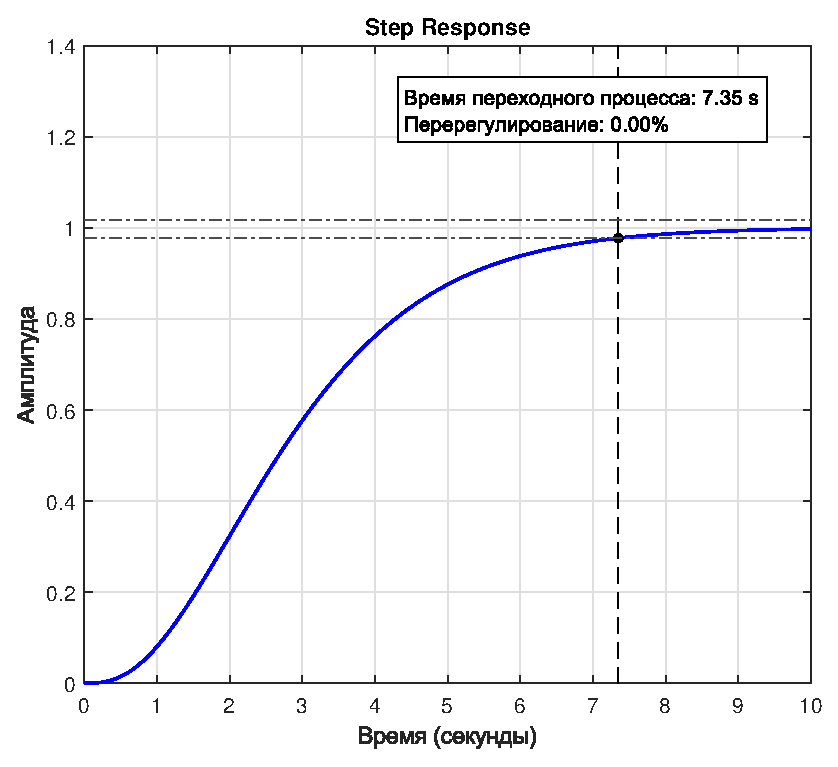
\includegraphics[width=\textwidth]{ex2/-1_-1_-1.eps}
        \caption{$\lambda_1=-1, \lambda_2=-1, \lambda_3=-1,$}
        \centerline{График переходного процесса}
    \end{minipage}\hfill
    \begin{minipage}{0.5\textwidth}
        \centering 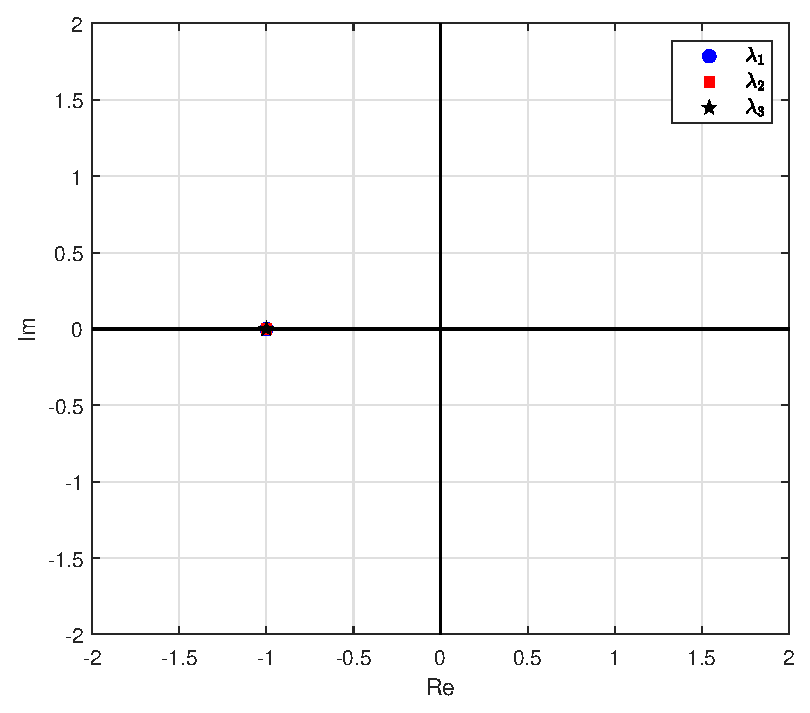
\includegraphics[width=\textwidth]{ex2/complex_plan_-1_-1_-1.eps}
        \caption{$\lambda_1=-1, \lambda_2=-1, \lambda_3=-1,$}
        \centerline{Выбранные корни на комплексной плоскости}
    \end{minipage}\\[1em]
\end{figure}\noindent\

По графику комплексной плоскости с отмеченными полюсами системы можно заметить, что все полюса расположены в одной точке, тогда они могут быть охвачены сколь угодно малым сектором, а значит их степень колебательности равна нулю, что и отображается на графике переходного процесса --- система не колеблется, стремится к установившемуся значению лишь снизу, не пересекая прямую $y = y_{\text{уст}}$. Значит, верхняя граница перерегулирования не подлежит оценке по связи со степенью колебательности ($e^{-\frac{\pi}{0}}\cdot 100\%$ не имеет значения из-за деления на 0). То же будет справедливо и для дальнейших вещественных наборов полюсов.

\begin{figure}[H]
    \begin{minipage}{0.5\textwidth}
        \centering 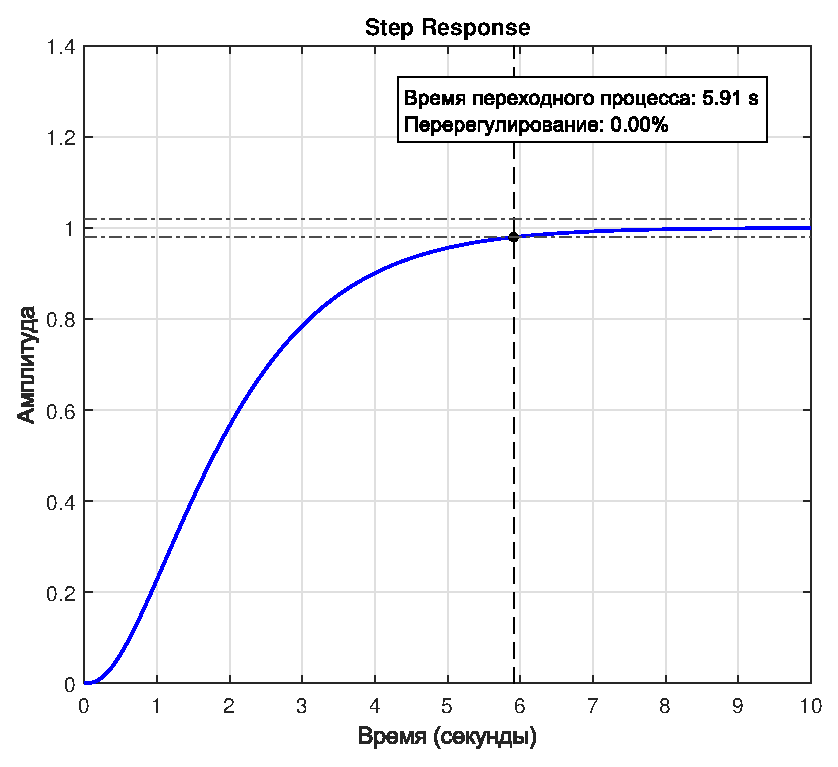
\includegraphics[width=\textwidth]{ex2/-1_-1_-10.eps}
        \caption{$\lambda_1=-1, \lambda_2=-1, \lambda_3=-10,$}
        \centerline{График переходного процесса}
    \end{minipage}\hfill
    \begin{minipage}{0.5\textwidth}
        \centering 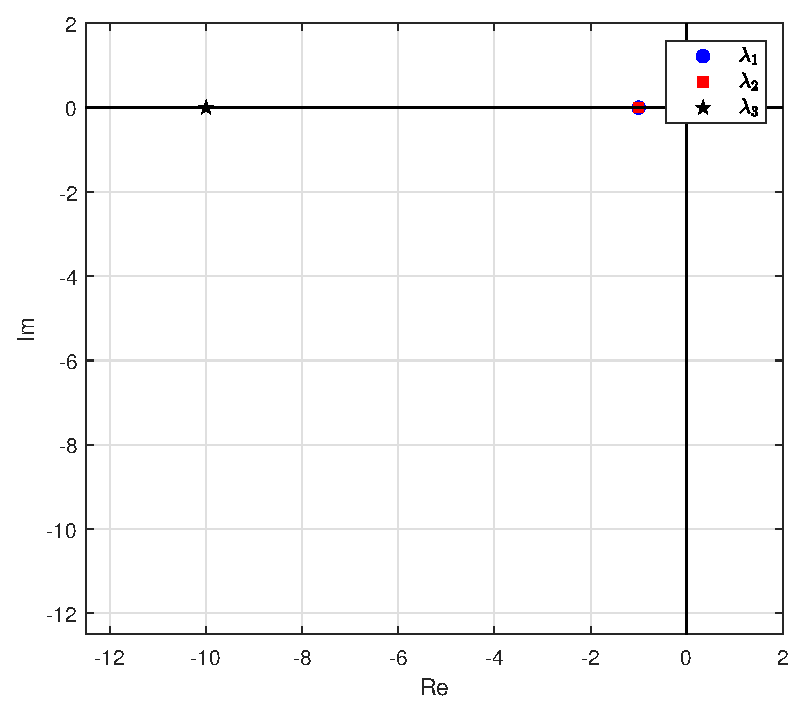
\includegraphics[width=\textwidth]{ex2/complex_plan_-1_-1_-10.eps}
        \caption{$\lambda_1=-1, \lambda_2=-1, \lambda_3=-10,$}
        \centerline{Выбранные корни на комплексной плоскости}
    \end{minipage}\\[1em]
\end{figure}\noindent\

Один из полюсов теперь располагается дальше по оси $\text{Im}$ на карте полюсов. Соответствующая ему мода затухает быстрее чем в первом случае, это и приводит к уменьшению времени переходного процесса. Перерегулирование всё также равно 0, как и степень колебательности.

\begin{figure}[H]
    \begin{minipage}{0.5\textwidth}
        \centering 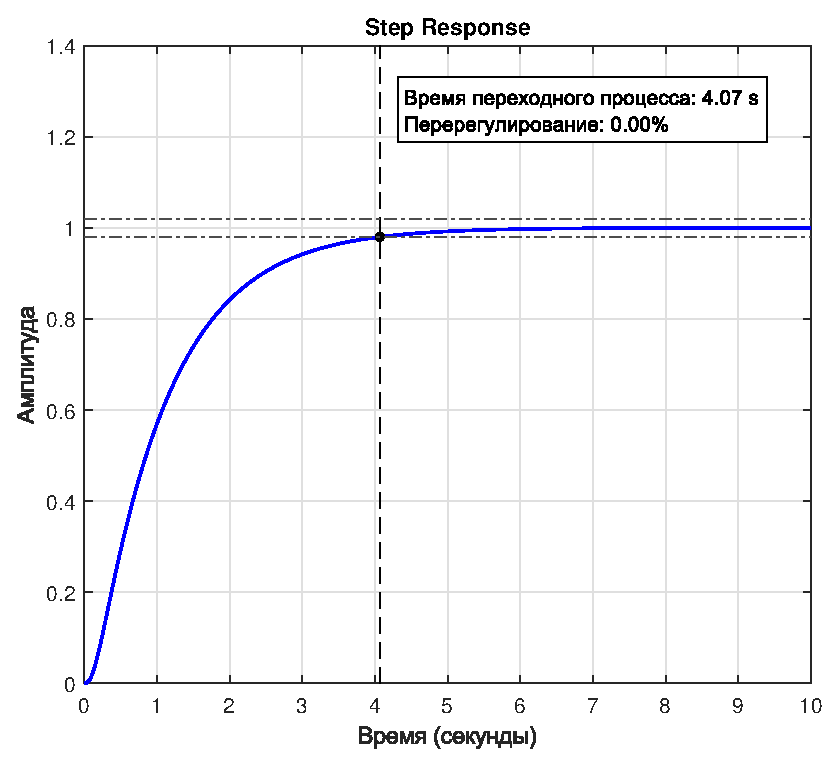
\includegraphics[width=\textwidth]{ex2/-1_-20_-10.eps}
        \caption{$\lambda_1=-1, \lambda_2=-20, \lambda_3=-10,$}
        \centerline{График переходного процесса}
    \end{minipage}\hfill
    \begin{minipage}{0.5\textwidth}
        \centering 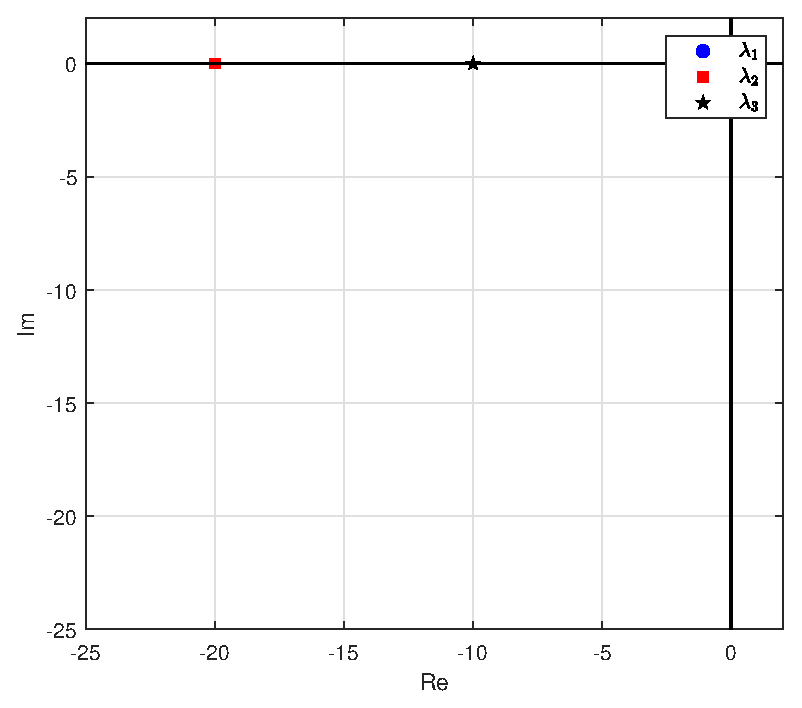
\includegraphics[width=\textwidth]{ex2/complex_plan_-1_-20_-10.eps}
        \caption{$\lambda_1=-1, \lambda_2=-20, \lambda_3=-10,$}
        \centerline{Выбранные корни на комплексной плоскости}
    \end{minipage}\\[1em]
\end{figure}\noindent\

Рассматривая графики для этого набора полюсов, видим, что время переходного процесса снова уменьшилось из-за увеличения значения одного из полюсов по модулю. Мнимой части корней всё также нет, из-за этого не наблюдается и колебательность.

\begin{figure}[H]
    \begin{minipage}{0.5\textwidth}
        \centering 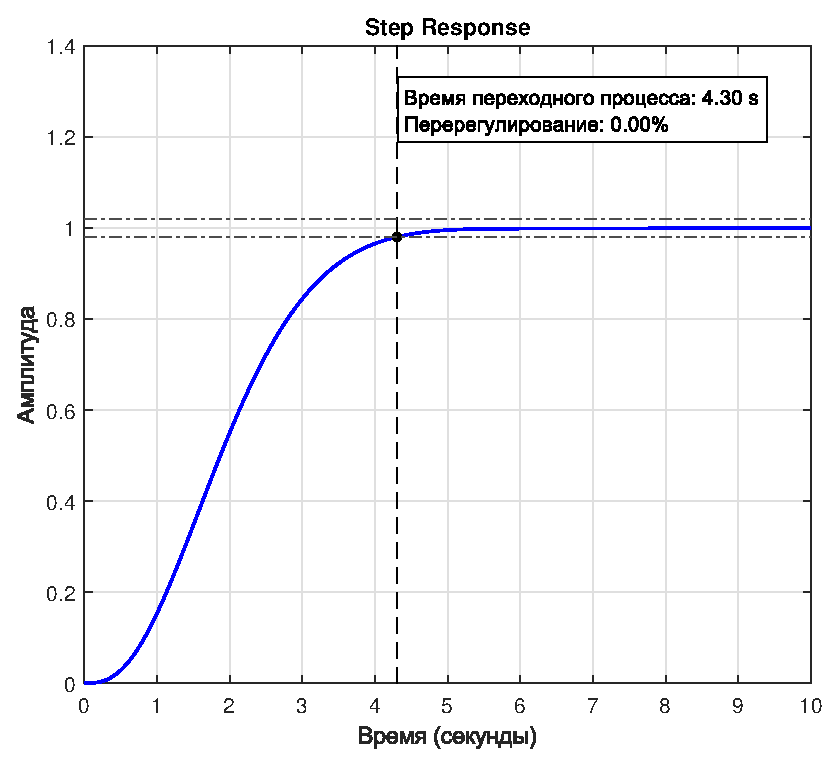
\includegraphics[width=\textwidth]{ex2/-1+1i_-1-1i_-1.eps}
        \caption{$\lambda_1=-1+i, \lambda_2=-1-i, \lambda_3=-1,$}
        \centerline{График переходного процесса}
    \end{minipage}\hfill
    \begin{minipage}{0.5\textwidth}
        \centering 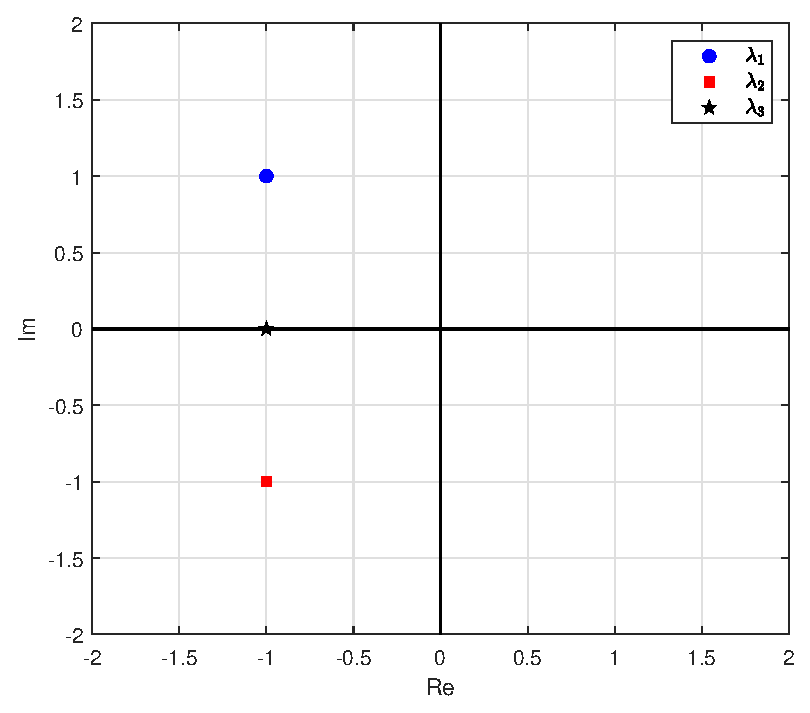
\includegraphics[width=\textwidth]{ex2/complex_plan_-1+1i_-1-1i_-1.eps}
        \caption{$\lambda_1=-1+i, \lambda_2=-1-i, \lambda_3=-1,$}
        \centerline{Выбранные корни на комплексной плоскости}
    \end{minipage}\\[1em]
\end{figure}\noindent\

В этом случае можно оценить степень колебательности и перерегулирование. По графику на комплексной плоскости можем заметить, что в предполагаемом секторе, в котором расположены полюса устойчивости системы, крайними полюсами являются $\lambda_1$ и $\lambda_2$. Степень колебательности определяется именно по ним: $\mu=\frac{|Im(\lambda_{2})|}{|Re(\lambda_{2})|}=\frac{1}{1}=1$. Тогда на основе полученного значения можно оценить верхнюю границу перерегулирования: $\sigma < e^{-\frac{\pi}{\mu}} \cdot 100\%= e^{-\frac{\pi}{1}} \cdot 100\% \approx 4.32 \%$. То есть в системе могут быть колебания вплоть до $4.32\%$ от установившегося значения. По графику переходного процесса можно заметить, что колебания отсутствуют вовсе. Это может быть связано с тем, что доминантный корень отсутствует --- все 3 полюса расположены на одинаковом расстоянии от оси $\text{Im}$.

\begin{figure}[H]
    \begin{minipage}{0.5\textwidth}
        \centering 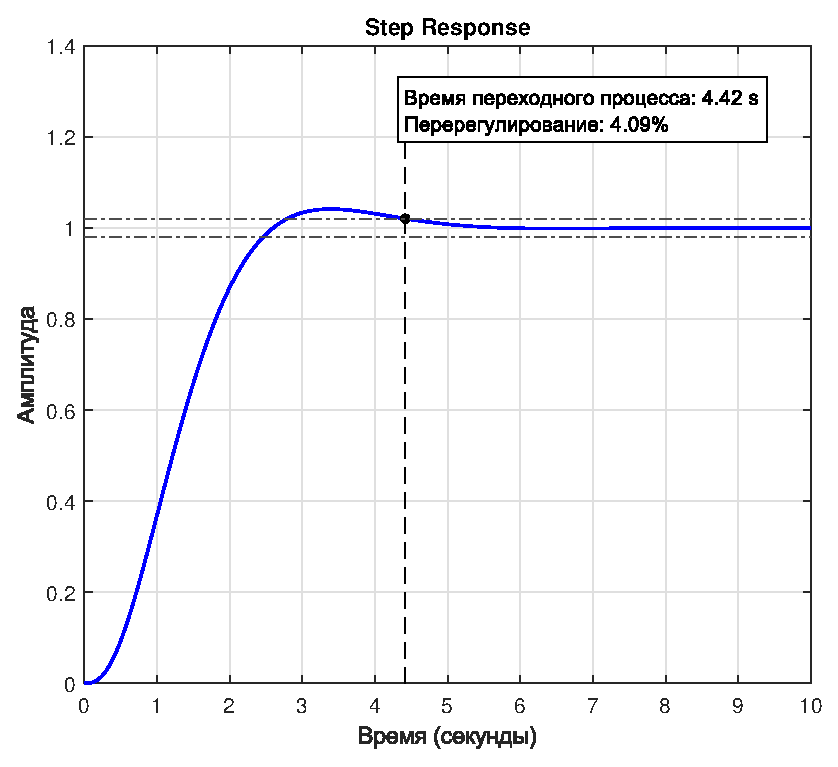
\includegraphics[width=\textwidth]{ex2/-1+1i_-1-1i_-5.eps}
        \caption{$\lambda_1=-1+i, \lambda_2=-1-i, \lambda_3=-5,$}
        \centerline{График переходного процесса}
    \end{minipage}\hfill
    \begin{minipage}{0.5\textwidth}
        \centering 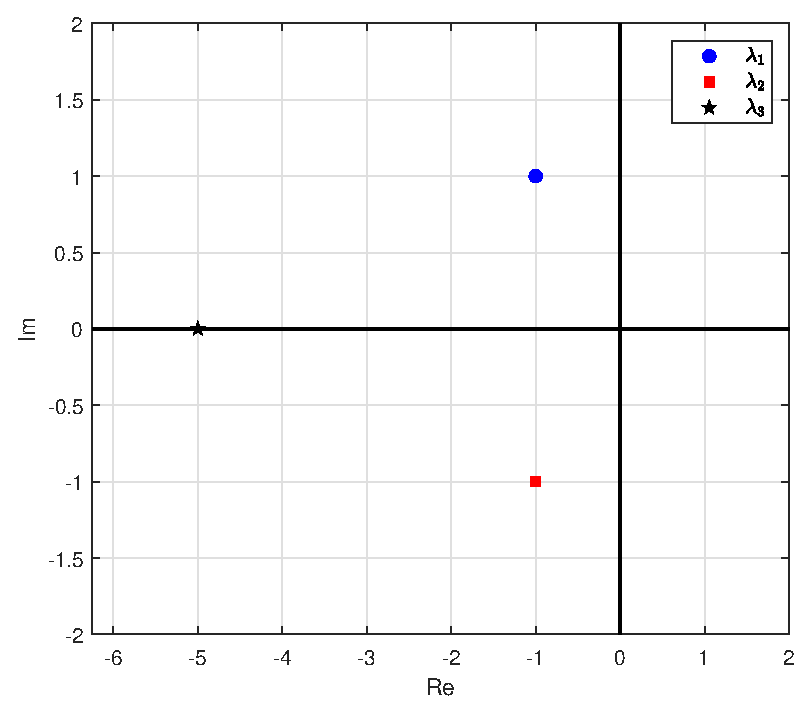
\includegraphics[width=\textwidth]{ex2/complex_plan_-1+1i_-1-1i_-5.eps}
        \caption{$\lambda_1=-1+i, \lambda_2=-1-i, \lambda_3=-5,$}
        \centerline{Выбранные корни на комплексной плоскости}
    \end{minipage}\\[1em]
\end{figure}\noindent\

Сразу оценим степень колебательности для этого случая. Крайними полюсами сектора являются всё те же $\lambda$, что и в прошлом случае, а значит, оценка верхней границы перерегулирования сохраняется --- $4.32\%$. Само же перерегулирование составило $4.09\%$, что меньше верхней его оценки. 

\begin{figure}[H]
    \begin{minipage}{0.5\textwidth}
        \centering 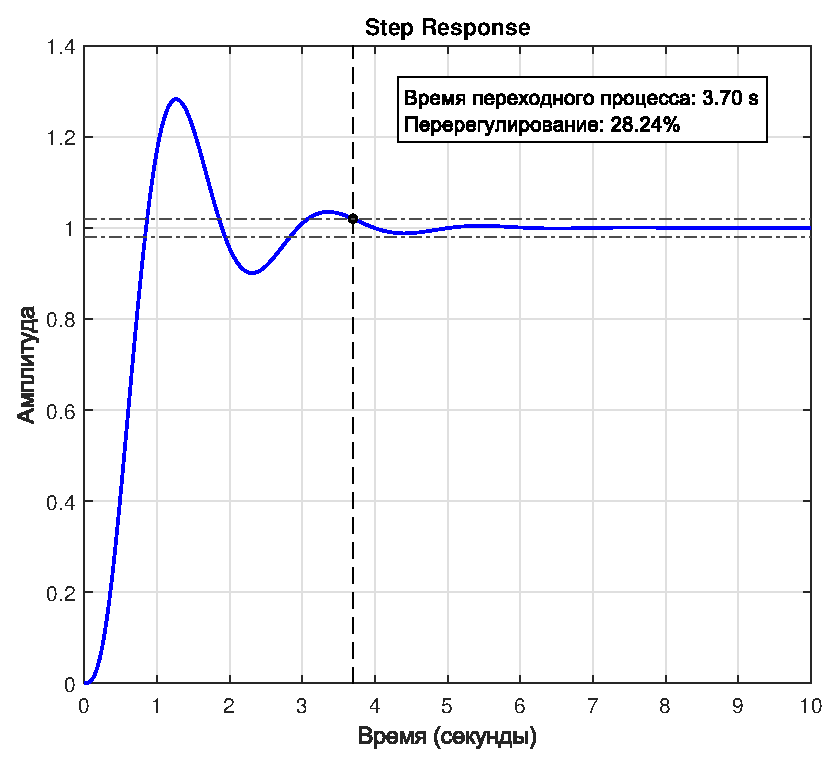
\includegraphics[width=\textwidth]{ex2/-1+3i_-1-3i_-5.eps}
        \caption{$\lambda_1=-1+3i, \lambda_2=-1-3i, \lambda_3=-5,$}
        \centerline{График переходного процесса}
    \end{minipage}\hfill
    \begin{minipage}{0.5\textwidth}
        \centering 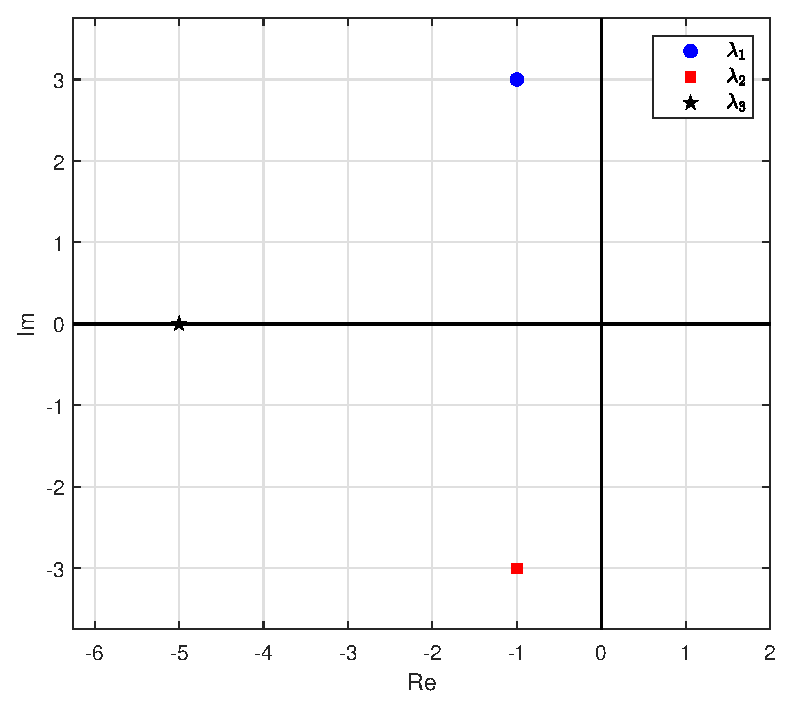
\includegraphics[width=\textwidth]{ex2/complex_plan_-1+3i_-1-3i_-5.eps}
        \caption{$\lambda_1=-1+3i, \lambda_2=-1-3i, \lambda_3=-5,$}
        \centerline{Выбранные корни на комплексной плоскости}
    \end{minipage}\\[1em]
\end{figure}\noindent\

В этом случае колебания системы гораздо сильнее из-за повышения значений мнимой части комплексных полюсов, однако время переходного процесса также ниже, почти на пятую часть.\

Степень колебательности всё также определяется по карте полюсов и равняется $3$. Рассчитаем по этому значению верхнюю оценку перерегулирования: $\sigma < e^{-\frac{\pi}{3}}\cdot 100\% \approx 35.092\%$. Верхняя граница довольно высокая в сравнении с предыдущими значениями. Найденное значение перерегулирования, $28.24\%$, не выходит за найденную верхнюю границу. 

\begin{figure}[H]
    \begin{minipage}{0.5\textwidth}
        \centering 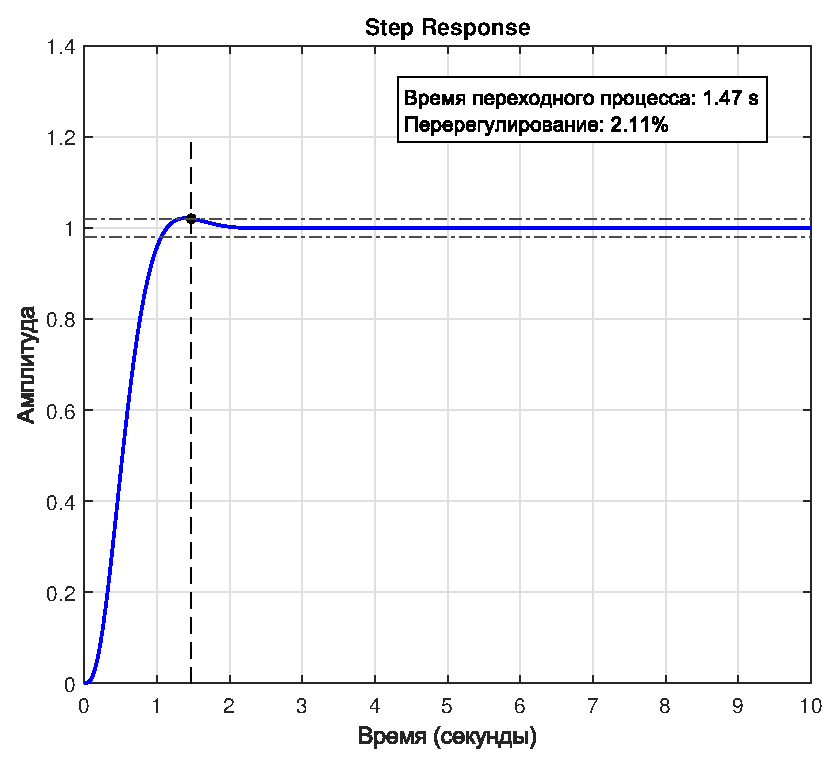
\includegraphics[width=\textwidth]{ex2/-3+3i_-3-3i_-5.eps}
        \caption{$\lambda_1=-3+3i, \lambda_2=-3-3i, \lambda_3=-5,$}
        \centerline{График переходного процесса}
    \end{minipage}\hfill
    \begin{minipage}{0.5\textwidth}
        \centering 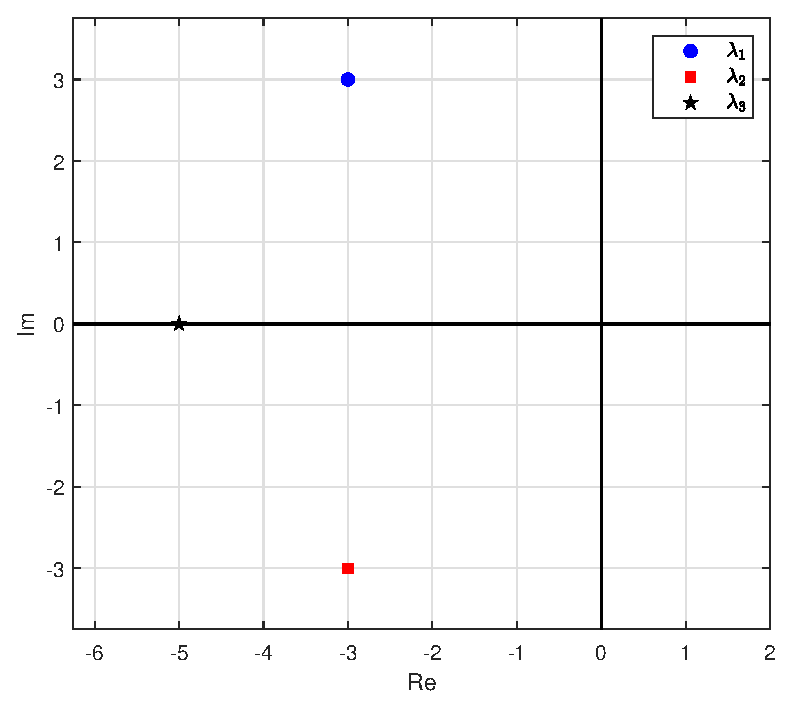
\includegraphics[width=\textwidth]{ex2/complex_plan_-3+3i_-3-3i_-5.eps}
        \caption{$\lambda_1=-3+3i, \lambda_2=-3-3i, \lambda_3=-5,$}
        \centerline{Выбранные корни на комплексной плоскости}
    \end{minipage}\\[1em]
\end{figure}\noindent\

И снова $\text{Re}(\lambda_{1,2})=\text{Im}(\lambda_{1, 2})$, что приводит к $\mu=1$, а $\sigma < 4.32\%$. Найденное значение перерегулирования ($2.11\%$) и в этом случае не больше верхней оценки. Время переходного процесса же сильно уменьшилось при увеличении модуля вещественной части комплексных корней.

\begin{figure}[H]
    \begin{minipage}{0.5\textwidth}
        \centering 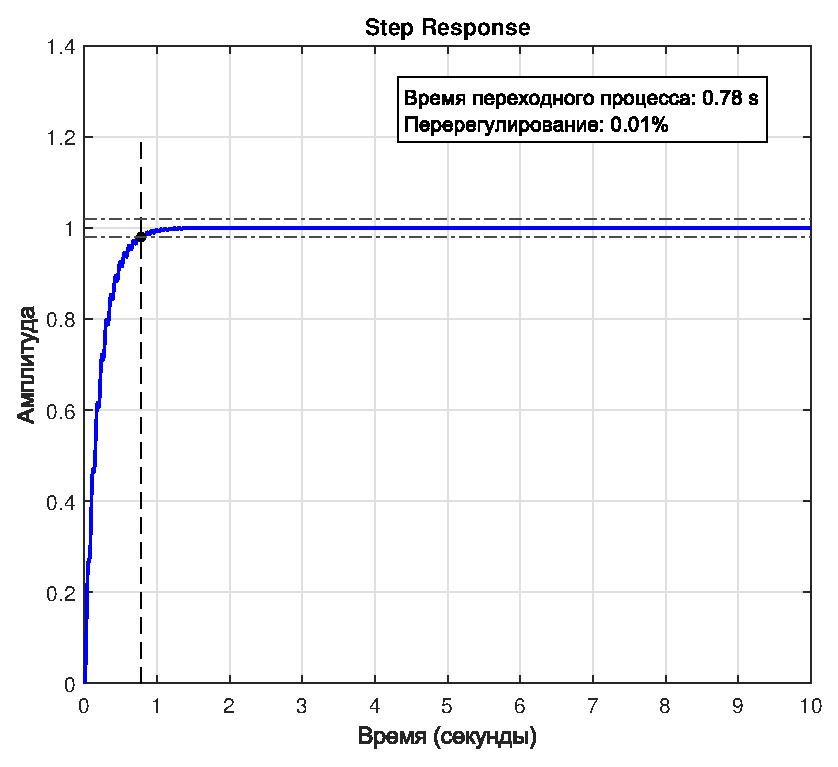
\includegraphics[width=\textwidth]{ex2/-3+100i_-3-100i_-5.eps}
        \caption{$\lambda_1=-3+100i, \lambda_2=-3-100i, \lambda_3=-5,$}
        \centerline{График переходного процесса}
    \end{minipage}\hfill
    \begin{minipage}{0.5\textwidth}
        \centering 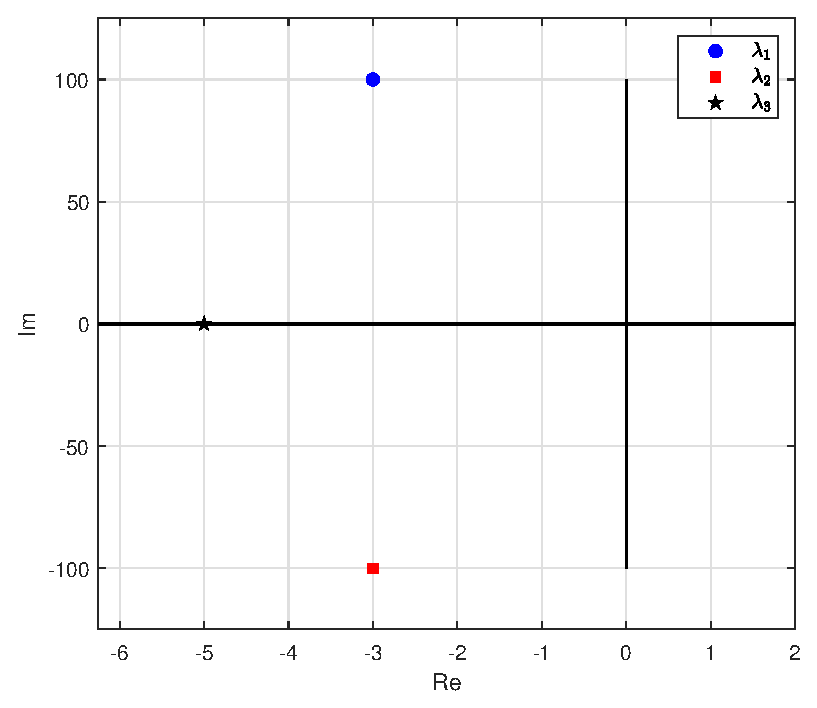
\includegraphics[width=\textwidth]{ex2/complex_plan_-3+100i_-3-100i_-5.eps}
        \caption{$\lambda_1=-3+100i, \lambda_2=-3-100i, \lambda_3=-5,$}
        \centerline{Выбранные корни на комплексной плоскости}
    \end{minipage}\\[1em]
\end{figure}\noindent\

Повышение значения мнимой части пары комплексно-сопряжённых полюсов по модулю привело к значительному увеличению числа периодов колебаний на рассматриваемом временном отрезке, и перерегулирование уменьшилось, как и время переходного процесса.\ 

Степень колебательности для этого случая равна $100/3$, и тогда верхняя оценка перерегулирования по связи со степенью колебательности: $\sigma < e^{-\frac{3\pi}{100}}\cdot 100\% \approx 91.005\%$.

\subsection{Выводы}

Чем выше располагаются полюса на карте полюсов, тем больше будет периодов колебаний на графике переходного процесса, обратно пропорционально колебательности при увеличении мнимой части комплексных корней меняется и время переходного процесса --- чем больше мнимая часть, тем быстрее система сходится к установившемуся значению. Можно достичь максимальной колебательности, а, соответственно, и максимального уменьшения времени переходного процесса, приблизив крайние комплексно-сопряжённые корни к прямой $\text{Re}=0$\.

При выполнении задания удалось ``погасить'' излишнюю колебательность за счёт увеличения вещественной части комплексно-сопряжённого полюса по модулю, уменьшив при этом время переходного процесса.

\section{Вывод по работе}\

Я познакомился с вынужденным движением, с тем, как именно входное воздействие влияет на выходы систем. Также ознакомился с показателями качества, которыми можно оценить составленную систему, на их основе подобрал наиболее оптимальные параметры для минимизации времени переходного процесса и перерегулирования, понял, в каких условиях вознакает перерегулирование, и как понять, каких значений оно может достичь.

\newpage

\section{Приложение А. Код для выполнения заданий}

\subsection*{Листинг 1. Код для выполнения задания 1}

\begin{lstlisting}[caption={Код для построения графиков для задания 1}, language=matlab]
% clear all;
close all;

[~, scriptName] = fileparts(mfilename('fullpath'));
if ~isfolder(scriptName)
    mkdir(scriptName);
end

t = (0:0.01:6)';
% u = [t, 1.5*ones(size(t))];
u = [t, 0.6*t];
% u = [t, sin(t*6)];
a_1 = -2;
a_0 = 65;
% u_str = '1.5';
u_str = '0.6t';
% u_str = 'sin(6t)';
y0 = 0;
y_t = figure;

for yy0 = [-1 0 1]
    out = sim('ex1/model.slx','StopTime','6');
    y_model = out.y;
    y_model.plot(DisplayName="$\dot{y}(0) = " + string(yy0) + ", y(0) = 0$", LineWidth=1.2)
    hold on;
end

legend(BackgroundAlpha=.99, Interpreter='latex', Location='best')
grid on;
title('$\ddot{y} + (' + string(a_1) + ')\dot{y} + (' + string(a_0) + ')y = ' + string(a_0) + 'u, u(t) = '+ u_str + '$', 'Interpreter', 'latex', FontWeight='normal')
xlabel('t'), ylabel('y(t)')
% ylim([-1.5, 1.5]);
saveas(y_t, string(scriptName) + '\'+u_str+'_' + string(a_1) + '_' + string(a_0) + '.eps', 'epsc')
\end{lstlisting}

\subsection*{Листинг 2. Код для выполнения задания 2}

\begin{lstlisting}[caption={Код для построения графиков для задания 2}, language=matlab]
% clear all;
close all;

t = (0:0.01:10)';
u = [t, ones(size(t))]; % входное воздействие -- функция Хевисайда

[~, scriptName] = fileparts(mfilename('fullpath'));
if ~isfolder(scriptName)
    mkdir(scriptName);
end

lambdas_all = [-1, -1, -1;
              -1, -1, -10;
              -1, -20, -10;
              -15, -20, -10;
              -1+1j, -1-1j, -1;
              -1+1j, -1-1j, -5;
              -1+3j, -1-3j, -5;
              -3+3j, -3-3j, -5;
              -1+1j, -1-1j, -15];

for i = 1:size(lambdas_all, 1)
    lambda1 = lambdas_all(i, 1);
    lambda2 = lambdas_all(i, 2);
    lambda3 = lambdas_all(i, 3);
    
    fig_complex = figure('Units', 'pixels', 'Position', [100 100 600 500]);
    hold on; grid on; box on;

    plot(real(lambda1), imag(lambda1), 'bo', 'MarkerFaceColor', 'b');
    plot(real(lambda2), imag(lambda2), 'red', 'Marker', 'square', 'MarkerFaceColor', 'red', 'LineStyle', 'none');
    plot(real(lambda3), imag(lambda3), 'black', 'Marker', 'pentagram', 'MarkerFaceColor', 'black', 'LineStyle', 'none');
    xlabel('Re'); ylabel('Im');

    plot([-100 100], [0 0], 'black', LineWidth=1.2)
    plot([0 0], [-100 100], 'black', LineWidth=1.2)
    legend('$\lambda_1$', '$\lambda_2$', '$\lambda_3$', 'Interpreter', 'latex', 'FontSize', 10);
    if (min(imag(lambdas_all(i, :))) ~= 0)
        ylim([min(-2, min(imag(lambdas_all(i, :)))-abs(min(imag(lambdas_all(i, :))))/4), max(2, max(imag(lambdas_all(i, :)))+abs(max(imag(lambdas_all(i, :))))/4)])
    else
        ylim([min(-2, min(real(lambdas_all(i, :)))-abs(min(real(lambdas_all(i, :)))/4)), max(2, max(real(lambdas_all(i, :)))+abs(max(real(lambdas_all(i, :))))/4)])
    end
    xlim([min(-2, min(real(lambdas_all(i, :)))-abs(min(real(lambdas_all(i, :))))/4), max(2, max(real(lambdas_all(i, :)))+abs(max(real(lambdas_all(i, :))))/4)])

    num = [abs(lambda3*lambda2*lambda1)];
    den = poly([lambda1, lambda2, lambda3]);
    sys = tf(num, den);
    y = lsim(sys, u(:,2), t);
    info = stepinfo(y, t);
    
    fig_main = figure('Units', 'pixels', 'Position', [100 100 600 500]);
    plot(t, y, LineWidth=1.3, Color='blue')
    grid on;
    title('Step Response')
    xlabel('Время (секунды)'), ylabel('Амплитуда')
    if (max(y) <= 1)
        ylim([0, 1.4])
    end
    hold on;
    y_final = info.SettlingMin + (info.SettlingMax - info.SettlingMin)/2; % среднее значение
    plot([info.SettlingTime info.SettlingTime], ylim, 'k--'); % вертикальная линия
    
    y_settle = interp1(t, y, info.SettlingTime);
    y_steady = y(end);               % установившееся значение
    y_difference = abs(y_steady - y_settle); % 0.02
    y_max = max(y);                  % максимум отклика
    yline(y_steady-y_difference, 'k-.'); % нижняя граница окрестности
    yline(y_steady+y_difference, 'k-.'); % верхняя граница окрестности
    sigma = abs(y_max - y_steady) / abs(y_steady) * 100;  % в процентах

    text('Units', 'normalized', ...
        'Position', [0.44 0.9], ...
        'String', sprintf('Время переходного процесса: %.2f s\nПеререгулирование: %.2f%%', info.SettlingTime, sigma), ...
        'BackgroundColor', 'w', ...
        'EdgeColor', 'k');

    % Отображаем точку
    plot(info.SettlingTime, y_settle, 'blacko', 'MarkerFaceColor', 'black', 'MarkerSize', 4);
    
    hold off;
    set(fig_complex, 'PaperUnits', 'inches', 'PaperPosition', [0 0 6 5]);
    saveas(fig_complex, string(scriptName) + '\complex_plan_' + string(lambda1) + '_' + string(lambda2) + '_' + string(lambda3) + '.eps', 'epsc')
    print(fig_main, '-depsc', string(scriptName) + '\' + string(lambda1) + '_' + string(lambda2) + '_' + string(lambda3) + '.eps')
    
end
\end{lstlisting}

\end{document}
